\documentclass[12pt]{article}

\usepackage{amsmath}
\usepackage{amssymb}
\usepackage{physics}
\usepackage{enumitem}
\usepackage{tikz}
\usetikzlibrary{arrows.meta,calc,angles,quotes}
\usepackage{geometry}
\geometry{margin=1in}

\setlength{\parindent}{0pt}

\begin{document}

{\Large \textbf{JEE Advanced Physics – Verified Set (Q1–Q15)}}\\[4pt]
\textbf{Single Correct Option}

\vspace{0.4cm}

\begin{enumerate}[label=\arabic*., leftmargin=0pt, itemindent=18pt, itemsep=1em]

%=========================================================
\item A uniform solid cylinder of mass $M$ and radius $R$ rolls without slipping inside a fixed vertical circular track of radius $3R$. The cylinder is released from rest from a height $h$ measured vertically from the lowest point of the track.

Using rolling constraint, conservation of mechanical energy, and radial force balance at the highest point, determine the minimum value of $h$ so that the cylinder just maintains contact at the top.

\begin{center}
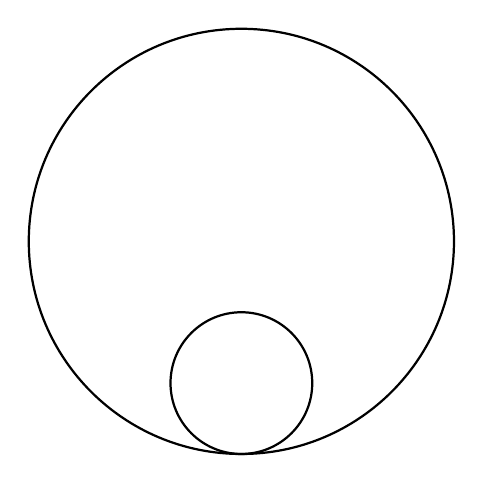
\begin{tikzpicture}[scale=0.9]
\draw[thick] (0,0) circle (3);
\draw[thick] (0,-2) circle (1);
\end{tikzpicture}
\end{center}

(A) $\frac{9R}{2}$  
(B) $\frac{11R}{2}$  
(C) $5R$  
(D) $6R$

%=========================================================
\item A wedge of mass $M$ rests on a smooth horizontal surface. A block of mass $m$ slides down its incline of angle $\theta$ without friction.

Using conservation of horizontal momentum and energy conservation, determine the horizontal acceleration of the wedge.

\begin{center}
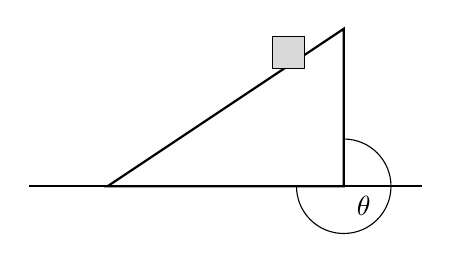
\begin{tikzpicture}[scale=1]

\coordinate (A) at (0,0);
\coordinate (B) at (5,0);
\coordinate (C) at (1,0);
\coordinate (D) at (4,0);
\coordinate (E) at (4,2);

\draw[thick] (A)--(B);
\draw[thick] (C)--(D)--(E)--cycle;

\draw pic["$\theta$", draw, angle radius=0.6cm]
{angle = C--D--E};

\draw[fill=gray!30] (3.1,1.5) rectangle (3.5,1.9);

\end{tikzpicture}
\end{center}

(A) $\frac{mg\sin\theta\cos\theta}{M+m}$  
(B) $\frac{mg\sin\theta\cos\theta}{M+m\sin^2\theta}$  
(C) $\frac{mg\sin\theta}{M+m}$  
(D) $\frac{mg\cos\theta}{M+m}$

%=========================================================
\item A particle of mass $m$ is released from rest at the top of a smooth fixed hemisphere of radius $R$. Let $\theta$ be the angle made by the radius vector of the particle with the vertical downward direction.

Using conservation of mechanical energy and radial force balance, determine the value of $\cos\theta$ at the instant the particle loses contact with the surface.

\begin{center}
\begin{tikzpicture}[scale=1]
\draw[thick] (0,0) arc (180:360:2);
\coordinate (O) at (0,0);
\coordinate (Top) at (0,2);
\coordinate (P) at ({2*sin(50)},{2*cos(50)});
\draw[dashed] (O)--(Top);
\draw[dashed] (O)--(P);
\draw pic["$\theta$",draw,angle radius=0.7cm]
{angle = Top--O--P};
\end{tikzpicture}
\end{center}

(A) $\frac{2}{3}$  
(B) $\frac{1}{2}$  
(C) $\frac{1}{3}$  
(D) $\frac{3}{4}$

%=========================================================
\item A conducting rod of length $L$ rotates with angular speed $\Omega$ about one end in a uniform magnetic field $B$ directed into the page.

Determine the potential difference between its ends.

\begin{center}
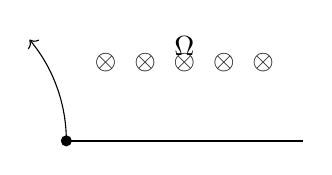
\begin{tikzpicture}[scale=1]
\draw[thick] (0,0)--(3,0);
\fill (0,0) circle (2pt);
\foreach \x in {0.5,1,1.5,2,2.5}
{\node at (\x,1){$\otimes$};}
\draw[->] (0,0) arc (0:40:2);
\node at (1.5,1.2) {$\Omega$};
\end{tikzpicture}
\end{center}

(A) $\frac{1}{2}B\Omega L^2$  
(B) $B\Omega L^2$  
(C) $\frac{1}{3}B\Omega L^2$  
(D) $\frac{1}{4}B\Omega L^2$

%=========================================================
\item A particle moves under the central potential
\[
V(r) = -\frac{k}{r} + \frac{\beta}{r^4},
\]
where $\beta>0$ and $\beta \ll k a^3$. For a nearly circular orbit of radius $a$, determine the magnitude of the apsidal advance per revolution to first order in $\beta$.

(A) $\frac{3\pi\beta}{k a^3}$  
(B) $-\frac{3\pi\beta}{k a^3}$  
(C) $\frac{2\pi\beta}{k a^3}$  
(D) $-\frac{2\pi\beta}{k a^3}$

%=========================================================
\item Two identical LC circuits each with inductance $L$ and capacitance $C$ are coupled by mutual inductance $M$.

Let $\omega_0=\frac{1}{\sqrt{LC}}$. Determine the normal mode frequencies.

(A) $\omega_0\sqrt{1\pm\frac{M}{L}}$  
(B) $\omega_0\left(1\pm\frac{M}{L}\right)$  
(C) $\omega_0\sqrt{1\pm\frac{M^2}{L^2}}$  
(D) $\omega_0\left(1\pm\frac{M^2}{L^2}\right)$

%=========================================================
\item An ideal gas rotates with angular speed $\Omega$ inside a cylindrical container at temperature $T$.

Determine the density variation with radial distance $r$.

(A) $\rho_0 e^{\frac{m\Omega^2 r^2}{2kT}}$  
(B) $\rho_0 e^{-\frac{m\Omega^2 r^2}{2kT}}$  
(C) $\rho_0 e^{\frac{m\Omega r}{kT}}$  
(D) $\rho_0 e^{-\frac{m\Omega r}{kT}}$

%=========================================================
\item A particle in a one-dimensional infinite potential well of width $L$ is subjected to perturbation $V(x)=\lambda x$.

Using first-order perturbation theory, determine the correction to ground state energy.

(A) $\frac{\lambda L}{2}$  
(B) $0$  
(C) $\frac{2\lambda L}{\pi^2}$  
(D) $\frac{\lambda L}{\pi}$

%=========================================================
\item A rigid body of moment of inertia $I$ rotates with angular speed $\omega_0$. A constant opposing torque $\tau$ acts.

Determine the angular displacement before it comes to rest.

(A) $\frac{I\omega_0^2}{2\tau}$  
(B) $\frac{I\omega_0}{\tau}$  
(C) $\frac{I\omega_0^2}{\tau}$  
(D) $\frac{\tau}{I\omega_0^2}$

%=========================================================
\item A charged particle moves through perpendicular electric field $E$ and magnetic field $B$.

Determine the velocity for which the particle passes undeflected.

(A) $\frac{E}{B}$  
(B) $EB$  
(C) $\frac{B}{E}$  
(D) $\frac{E}{B^2}$

%=========================================================
\item Monochromatic light of frequency $\nu$ is incident on a metal surface of work function $\phi$. The emitted electrons (charge magnitude $e$) move toward a collector through a region of uniform electric field $E$ directed opposite to their initial velocity. The electric field exists only over a distance $d$ between the emitter and collector.

Assuming the most energetic electrons just reach the collector with zero final speed, determine the minimum frequency $\nu$ required.

(A) $\nu = \frac{\phi + eEd}{h}$  
(B) $\nu = \frac{\phi - eEd}{h}$  
(C) $\nu = \frac{eEd}{h}$  
(D) $\nu = \frac{\phi}{h}$

%=========================================================
\item A conductor consists of a circular arc of radius $R$ subtending an angle $\theta$ (in radians) at its centre $O$. The arc is connected to two semi-infinite straight wires that are tangential to the arc at its ends. A steady current $I$ flows from one straight wire into the arc and then out through the other straight wire, as shown.

Determine the magnitude of the magnetic field at the centre $O$.

\begin{center}
\begin{tikzpicture}[scale=1]

\coordinate (O) at (0,0);
\coordinate (A) at (2,0);
\coordinate (B) at (-1,1.732);

\draw[thick] (A) arc (0:120:2);
\draw[thick] (A)--(4,0);
\draw[thick] (B)--(-3,1.732);

\draw[->] (3,0)--(3.6,0);
\draw[->] (-2.4,1.732)--(-2.9,1.732);

\fill (O) circle (2pt);
\node[below] at (O) {$O$};

\draw pic["$\theta$", draw, angle radius=0.8cm]
{angle = A--O--B};

\end{tikzpicture}
\end{center}

(A) $\frac{\mu_0 I}{4\pi R}(\theta + 2)$  
(B) $\frac{\mu_0 I}{4\pi R}(\theta - 2)$  
(C) $\frac{\mu_0 I}{4\pi R}\theta$  
(D) $\frac{\mu_0 I}{2\pi R}(\theta + 1)$

%=========================================================
\item A particle of positive charge $q$ and mass $m$ enters a region with initial horizontal velocity $v$ toward the right. A uniform electric field $\vec{E}$ acts vertically upward. A uniform magnetic field $\vec{B}$ acts perpendicular to the page (into the page). Gravity acts vertically downward with acceleration $g$.

Determine the value of $v$ for which the particle moves in a straight horizontal line without vertical deflection.

\begin{center}
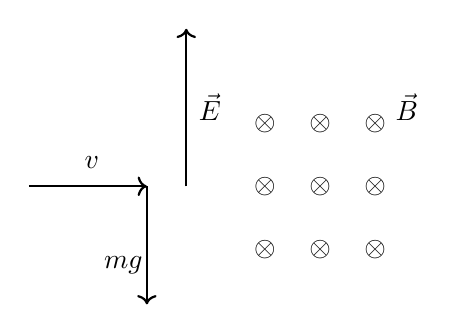
\begin{tikzpicture}[scale=1]
\draw[->,thick] (-2,0)--(-0.5,0);
\node at (-1.2,0.3) {$v$};
\draw[->,thick] (0,0)--(0,2);
\node at (0.3,1) {$\vec{E}$};
\foreach \x in {1,1.7,2.4}
\foreach \y in {-0.8,0,0.8}
\node at (\x,\y){$\otimes$};
\node at (2.8,1) {$\vec{B}$};
\draw[->,thick] (-0.5,0)--(-0.5,-1.5);
\node at (-0.8,-1) {$mg$};
\end{tikzpicture}
\end{center}

(A) $\frac{E - \frac{mg}{q}}{B}$  
(B) $\frac{E + \frac{mg}{q}}{B}$  
(C) $\frac{E}{B}$  
(D) $\frac{mg}{qB}$

%=========================================================
\item In Young’s double slit experiment, a thin glass slab of thickness $t$ and refractive index $\mu$ is introduced in front of one slit. Wavelength in air is $\lambda$.

Determine the shift in central fringe position on the screen at distance $D$.

(A) $\frac{D(\mu -1)t}{d}$  
(B) $\frac{D\mu t}{d}$  
(C) $\frac{(\mu -1)t}{d}$  
(D) $\frac{D(\mu -1)t}{\lambda}$

%=========================================================
%=========================================================
\item In Young’s double slit experiment, monochromatic light of wavelength $\lambda$ is used and the slits are separated by distance $d$. The screen is placed at distance $D$ ($D \gg d$). A thin transparent sheet of refractive index $\mu$ and uniform thickness $t$ is placed in front of one slit.

Now, in addition, the entire apparatus is immersed in a liquid of refractive index $\mu_0$ ($\mu_0 < \mu$). The wavelength of light in the liquid becomes $\lambda_0 = \frac{\lambda}{\mu_0}$.

Determine the new fringe width on the screen.

(A) $\displaystyle \frac{\lambda D}{d}$  

(B) $\displaystyle \frac{\lambda D}{\mu_0 d}$  

(C) $\displaystyle \frac{\lambda D}{\mu_0^2 d}$  

(D) $\displaystyle \frac{\lambda D}{d} \left( \frac{\mu}{\mu_0} \right)$

\end{enumerate}

\end{document}